\chapter{System Implementation}

The product of this thesis is a prototype website for counselors with topic model
visualizations in addition to the core Crisis Text Line functionality. In this chapter,
we describe each component integrated into the system and the variety of
technologies used to assist in development.

\section{Front-End Website}

\begin{figure}[h]
  \centering
    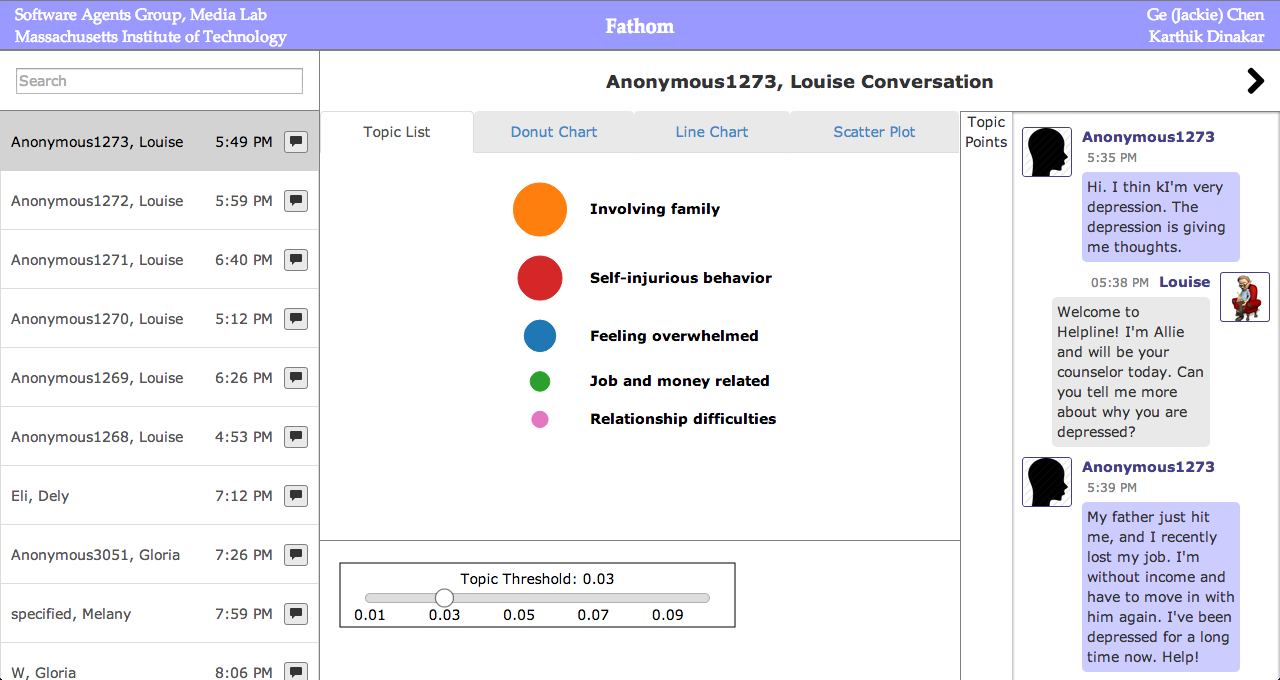
\includegraphics[width=\textwidth]{website.png}
  \caption{This screenshot is a complete view of the prototype website with topic
  model visualizations.}
  \label{website}
\end{figure}

The front-end was built for the Chrome browser using HTML, CSS, and JavaScript
with the help of jQuery \cite{jquery}, the JavaScript library, and Bootstrap \cite{bootstrap}, a front-end
framework or web projects. It has not been tested with other browsers because this
project is only a prototype, and the CTL framework mostly uses Chrome as well.
Figure~\ref{website} shows a complete view of the webpage. On the left is a searchable, scrollable
list of conversations, and on the right is the conversation view. The conversation view
has a title header on top with previous and next arrows for navigation between
conversations, tabs for the four visualizations on the left, and the conversation transcript
on the right.

\begin{figure}[h]
  \centering
    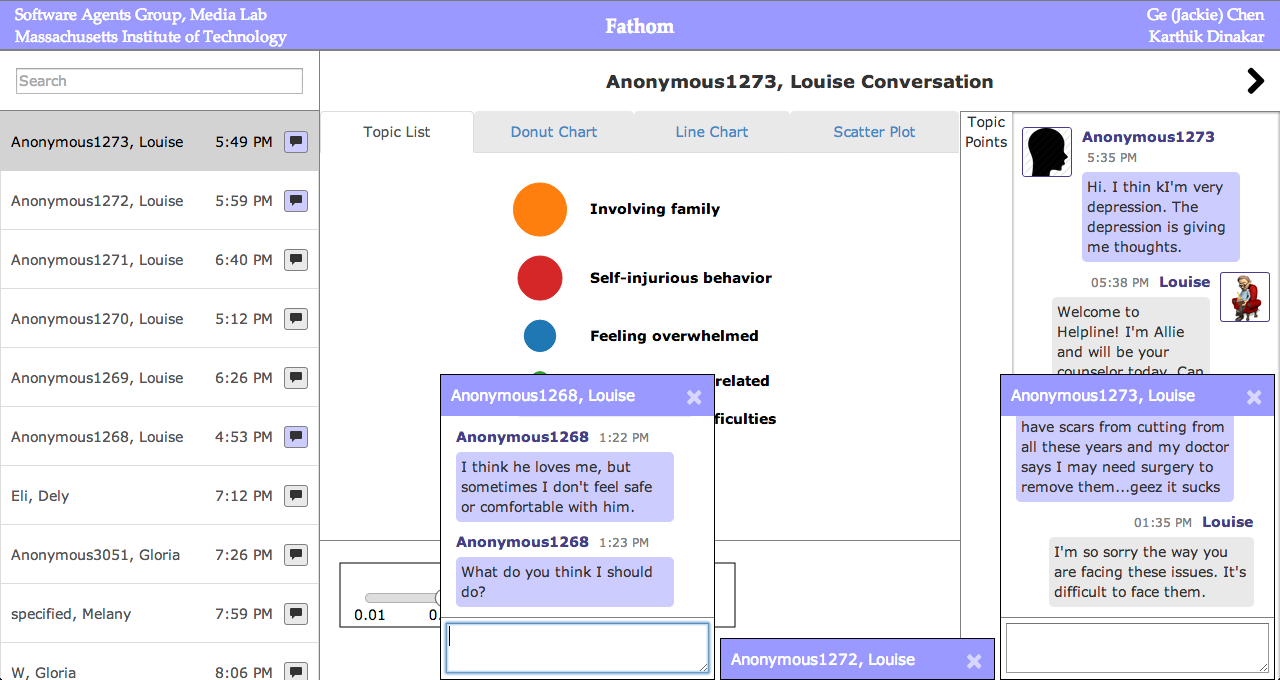
\includegraphics[width=\textwidth]{chatbox.png}
  \caption{The website has typical chat functionality so counselors can handle
  incoming text messages from clients.}
  \label{chatbox}
\end{figure}

As shown in Figure~\ref{chatbox}, the list of conversations also acts as a chat list. Clicking
on the chat icon for a conversation will open a typical chat box. The title in the chat
box header is a link to the view for that conversation. Chat boxes can be minimized
or closed by clicking on the header. Typing text into the text area and hitting the
Enter key will send a message as the counselor for the corresponding conversation.

The website was designed from scratch following good user interface practices
such as efficiency, learnability, and consistency. Navigation between conversations
is efficient with search functionality, previous/next arrows, and links in the chat box
headers. Typical elements such as the scrolling list and chat boxes have behavior that
is consistent with external applications. The interface is simple in terms of layout
and color with no extraneous elements.

\section{Back-End Server and Database}

The back-end uses Flask \cite{flask}, a framework for Python web development, and the data
is stored in a mySQL database \cite{mysql}. Flask runs a simple development server with an
easy API for handling requests, which made it suitable for our prototype development.
The website is served using a single url, with additional communication between the
front-end and back-end done through AJAX calls with Flask routing. A Python class
was created to interact with mySQL and process the data going into and out of the
database.

\section{Topic Model Data}

Karthik Dinakar developed the topic model for our conversation summaries using a
labeled mixed-initiative latent dirichlet allocation (L-LDA) approach. The model was
trained using a dataset of 881,901 messages between counselors and clients from CTL.
With this computational model, he wrote a function that takes a message as input and
outputs the topics and proportions associated with the words in that message. We
run this function on all client messages in the database, as well as any new messages,
and store the output in an additional column in the database.

The visual indexing visualizations use the topic model data directly in the output
format described, with a set of topics and proportions for each message. Topics may
be filtered out if the corresponding proportions are below a given threshold. For the
visual summary visualizations, we combine the data from all client messages in a
given conversation by normalizing the proportions for each topic across the messages.

\section{Visualizations}

With the topic model data in the formats described above, the four designed
visualizations were developed using D3, a JavaScript library for creating SVG visualizations
based on data \cite{d3, d3website}. D3 is a great framework for this thesis because the visualizations
are built around the data as input. As the topic model data changes between
conversations or with new messages, no additional code is written. The framework
also has examples online, as well as tools for updating the graphics with smooth transitions.

The topic list visualization was programmed based on D3 examples of a legend.
Similarly, the donut chart, multi-series line chart, and scatter plot all have example
code to follow to learn the framework. With new topic model data, the summary
visualizations are completely redrawn. The indexing visualizations transition the axes
and points as new messages are received, since they are time-based. All visualizations
update dynamically in real-time, so they can be used for ongoing conversations.

For visual indexing, the line chart and scatter plot also perform AJAX calls.
The first time a topic is selected for a conversation, the front-end sends the HTML
positions of the client messages in the transcript to the server, and the server retrieves
the message tags for the \textbf{Topic Points} column. Only the tags for the selected topic
are shown; the other tags are in the HTML document but hidden.

\begin{figure}[h]
  \centering
    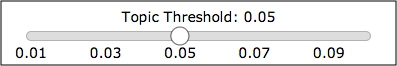
\includegraphics[width=0.7\textwidth]{slider.png}
  \caption{This liberal to conservative meter allows the user to choose the threshold
  for filtering topic proportions based on how many topics they would like to see.}
  \label{slider}
\end{figure}

The last aspect of the D3 work is the \textbf{Topic Threshold} slider in Figure~\ref{slider}. This
slider allows the user to change the threshold for filtering topics based on proportions,
acting as a liberal to conservative meter. Decreasing the threshold shows more topics
with lower proportions, while increasing the threshold shows fewer topics. Changes
are updated for all visualizations in real-time.

\section{Texting Integration}

Finally, Twilio \cite{twilio} was used to simulate the CTL functionality of clients sending
text messages that are received by counselors in chat form. Twilio has a text messaging
API that allows web applications to send and receive SMS messages. Integrating text
messages required some nontrivial changes to our front-end and back-end.

When a text message is received as a request by the server, the server needs to
communicate this information to the front-end client. There are a number of ways to
do this, such as web sockets, server-side events, long-polling, or additional
frameworks. We chose to implement long-polling to minimize the use and integration
of extraneous technologies. The idea of long-polling is to keep an open connection
between the server and client until the server has information to send to the client.
We implement this by having the client make a request to the server as soon as it
loads. When this request is received by the server, the server checks if there is new
information to send to the client. If there is a new text message with updated topic
model data, the server completes the request and the client immediately polls the
server again when it receives the response. Otherwise if there is no new data, the
server sleeps for a second and checks for new information again in a continuous loop.

By default, Flask's development server handles only one request at a time. To
be able to serve the website, perform long-polling, and receive text messages through
Twilio simultaneously, we chose to make the Flask application multi-threaded instead
of switching to a deployment framework that handles multiple requests at once. The
mySQL database access points then required locking to be thread-safe.

Besides these additions, the rest of the changes were expected. When a text
message is received, the database is checked to see whether the text is for an old or
new conversation. New conversations are added to the conversation list. If the chat
box for the conversation is already open, the messages must be updated. Otherwise
the chat box must open automatically. If the view for this conversation is shown,
the visualizations must be updated. Finally, any message added through the web
interface by the counselor must be sent to the client's phone number using Twilio.
